\documentclass[12pt,a4paper]{report}
\usepackage[utf8]{inputenc}
\usepackage[T1]{fontenc}
\usepackage{graphicx}
\usepackage[margin=1in]{geometry}
\usepackage{float}
\usepackage{titlesec}
\usepackage{caption}
\usepackage{fancyhdr}
\usepackage{hyperref}
\usepackage{booktabs}
\usepackage{xcolor}
\usepackage{amsmath}
\usepackage{amssymb}
\usepackage{amsfonts}
\usepackage{mathtools}
\usepackage{physics}

\titleformat{\chapter}[display]{\normalfont\huge\bfseries}{\chaptertitle}{20pt}{\Huge}
\pagestyle{fancy}
\fancyhf{}
\fancyhead[R]{\thepage}
\fancyhead[L]{\leftmark}
\renewcommand{\headrulewidth}{0.4pt}

\begin{document}

\begin{titlepage}
\begin{center}
{\Huge\bfseries Comparative Analysis of TCP Variants\\[1.5cm]}
{\Large\bfseries Performance Evaluation of Traditional and Enhanced TCP Implementations\\[1cm]}
\vfill
{\large Technical Report\\[0.5cm]}
{\large Network Performance Analysis Group\\[0.5cm]}
{\large \today}
\end{center}
\end{titlepage}

\tableofcontents
\newpage

\chapter{Introduction}
\section{Background}
This report presents a detailed comparative analysis of various TCP variants, focusing on traditional implementations and their enhanced versions. The study examines the performance characteristics and behavioral patterns of different TCP variants under controlled network conditions.\n

\chapter{Methodology}
\section{Experimental Setup}
The analysis was conducted using the ns-3 network simulator with the following configuration:
\begin{itemize}
\item Multiple concurrent TCP flows (0-6)
\item Controlled network conditions for consistent comparison
\item Comprehensive metric collection including cwnd, RTT, RTO
\item Data averaging across flows for statistical significance
\end{itemize}

\section{Metrics Analyzed}
\begin{itemize}
\item Congestion Window (cwnd): Measures the sending rate adaptation
\item Round Trip Time (RTT): Indicates network latency
\item Retransmission Timeout (RTO): Shows congestion response
\item In-Flight Packets: Represents active network utilization
\item Slow Start Threshold (ssth): Indicates congestion control transitions
\end{itemize}
\newpage\section{Proposed Variant of Westwood+}
\subsection{Intuition}
The traditional TCP Westwood+ algorithm uses a fixed value of $\alpha$ for all flows in the network. However, this leads to similar congestion window growth patterns across different flows, potentially causing synchronized packet losses. Our proposed variant introduces stochastic behavior by varying $\alpha$ according to a normal distribution, leading to more diverse congestion window growth patterns across flows.

\subsection{Mathematical Proof}
From the plot it is evident that, the time after which the incrementing portion reaches a steady state is important, since near that point, the cwnd tends to drop due to packet loss. One issue with the traditional algorithms is that, this time is roughly being the same for all the flows in the network since, we are using the same value of $\alpha$ for every node.

We now proceed to express this time $T$, taken to reach an approximately steady state from the initial state in terms of $\alpha$. Then we will use that relation to derive the distribution of the chosen value of $\alpha$, which leads to our desired distribution of the time $T$.
\begin{equation*}
W \leftarrow W + \frac{W_{max} - W}{\alpha W}
\end{equation*}

To model this simply, let us assume $W_{max} = k$ and that we are starting at $t = 0$ with $W = \frac{k}{3}$
\begin{equation*}
\text{Now,} \quad \frac{dW}{dt} = \frac{k-W}{\alpha W}
\end{equation*}
\begin{equation*}
\Rightarrow \frac{W dW}{k-W} = \frac{dt}{\alpha}
\end{equation*}
\begin{equation*}
\Rightarrow \int \frac{W dW}{k-W} = \int \frac{dt}{\alpha}
\end{equation*}

Now, assume we want to find the time to reach from $\frac{k}{3}$ to $\frac{9k}{10}$ [since reaching exactly $k$ is not possible in finite time, in fact packet loss will occur before that]
\begin{equation*}
\text{So,} \quad \int_{\frac{k}{3}}^{\frac{9k}{10}} \frac{W dW}{k-W} = \int_{0}^{T} \frac{dt}{\alpha}
\end{equation*}
\begin{equation*}
\Rightarrow -\int_{\frac{k}{3}}^{\frac{9k}{10}} \left(1 - \frac{k}{k-W}\right) dW = \frac{T}{\alpha}
\end{equation*}
\begin{equation*}
\Rightarrow \left[W + k\ln|k-W|\right]_{\frac{k}{3}}^{\frac{9k}{10}} = -\frac{T}{\alpha}
\end{equation*}
\begin{equation*}
\Rightarrow T = -\alpha\left[\frac{17}{30}k - 1.897k\right]
\end{equation*}
\begin{equation*}
\Rightarrow T = 1.3305\alpha k
\end{equation*}
\begin{equation*}
\Rightarrow T = 1.3305\alpha W_{max}
\end{equation*}

Therefore, regardless of our assumptions about the initial and stopping conditions, T is always directly proportional to our choice of $\alpha$
\begin{equation*}
T \propto \alpha
\end{equation*}

Thus, to enforce that time $T$ varies according to a normal distribution, we also need to enforce that $\alpha$ follows a normal distribution across different flows.
\newpage
\chapter{Results and Analysis}
\section{TCP Veno vs TCP Westwood+}
\noindent Comparison of the base TCP Veno and TCP Westwood+ variants.


\newpage
\subsection{Congestion Window}
\begin{figure}[H]
\centering
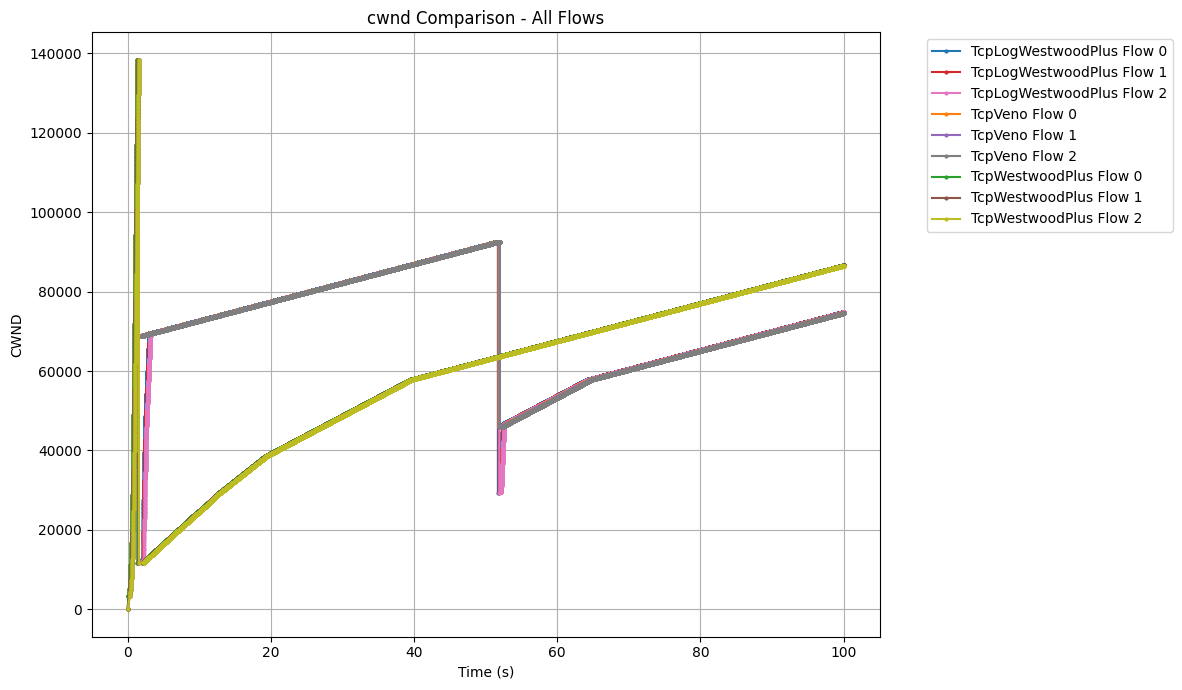
\includegraphics[width=0.95\textwidth]{plots/combined/Veno-WestwoodPlus/flowcombined/cwnd_all_flows_comparison.png}
\caption{Congestion Window Analysis for TCP Veno vs TCP Westwood+}
\label{fig:Veno-WestwoodPlus_cwnd}
\end{figure}

\newpage

\newpage
\subsection{In-Flight Packets}
\begin{figure}[H]
\centering
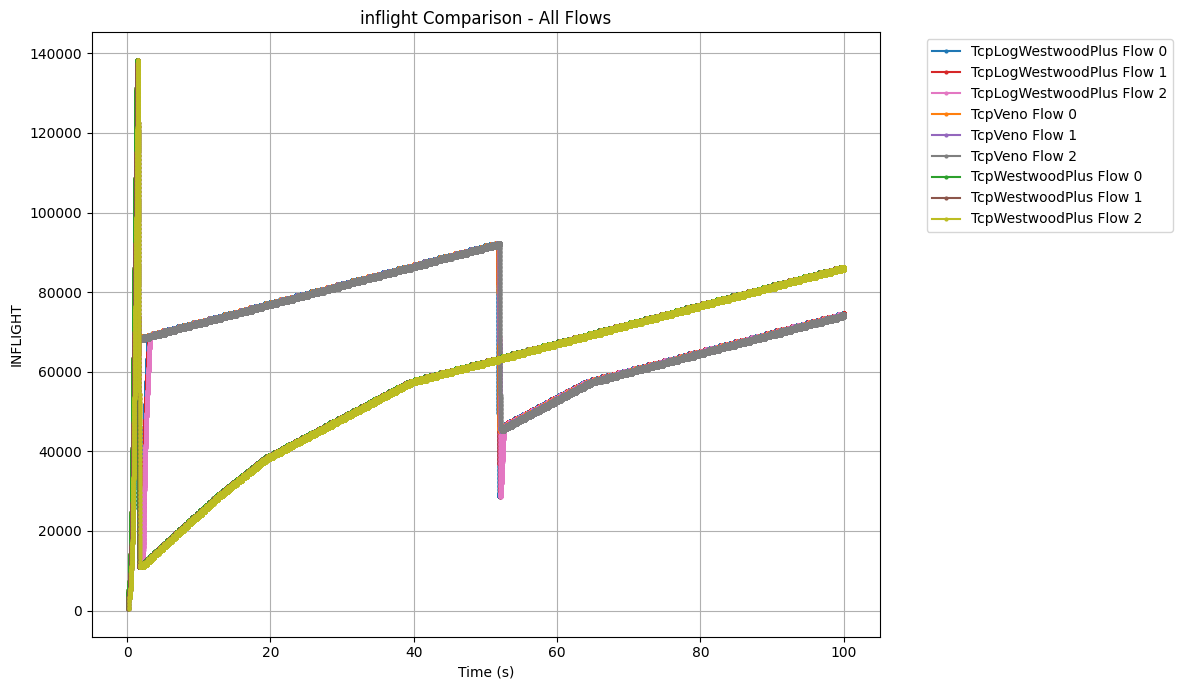
\includegraphics[width=0.95\textwidth]{plots/combined/Veno-WestwoodPlus/flowcombined/inflight_all_flows_comparison.png}
\caption{In-Flight Packets Analysis for TCP Veno vs TCP Westwood+}
\label{fig:Veno-WestwoodPlus_inflight}
\end{figure}

\newpage

\newpage
\subsection{Next RX}
\begin{figure}[H]
\centering
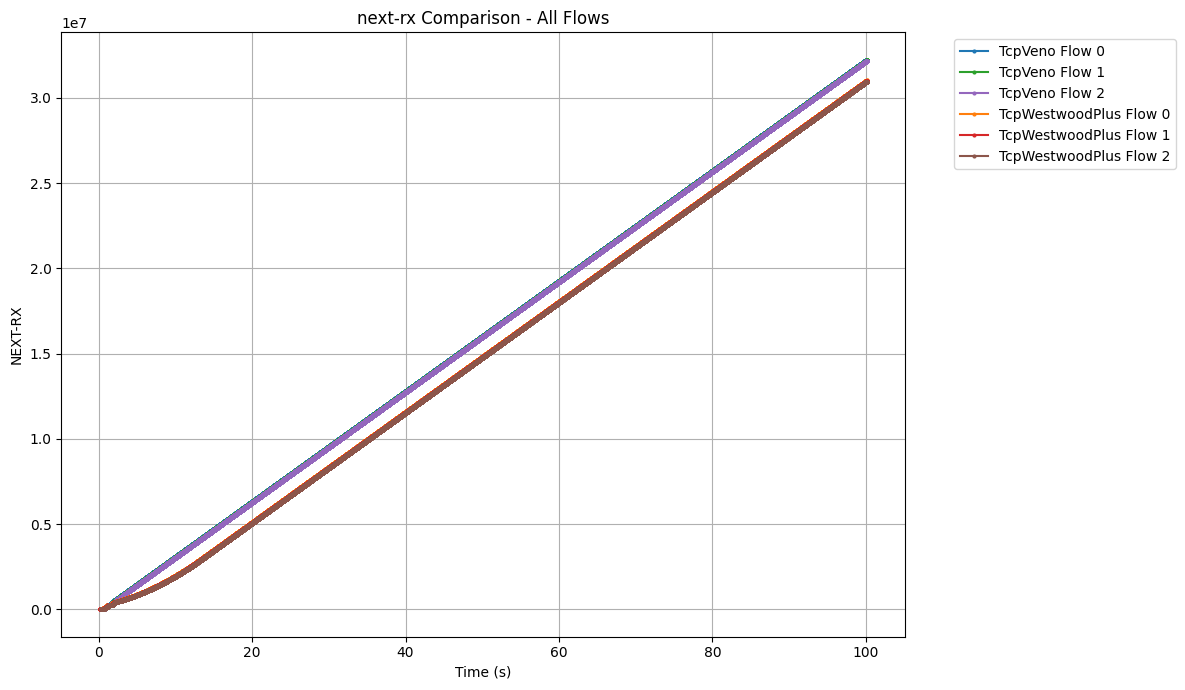
\includegraphics[width=0.95\textwidth]{plots/combined/Veno-WestwoodPlus/flowcombined/next-rx_all_flows_comparison.png}
\caption{Next RX Analysis for TCP Veno vs TCP Westwood+}
\label{fig:Veno-WestwoodPlus_next-rx}
\end{figure}

\newpage

\newpage
\subsection{Next TX}
\begin{figure}[H]
\centering
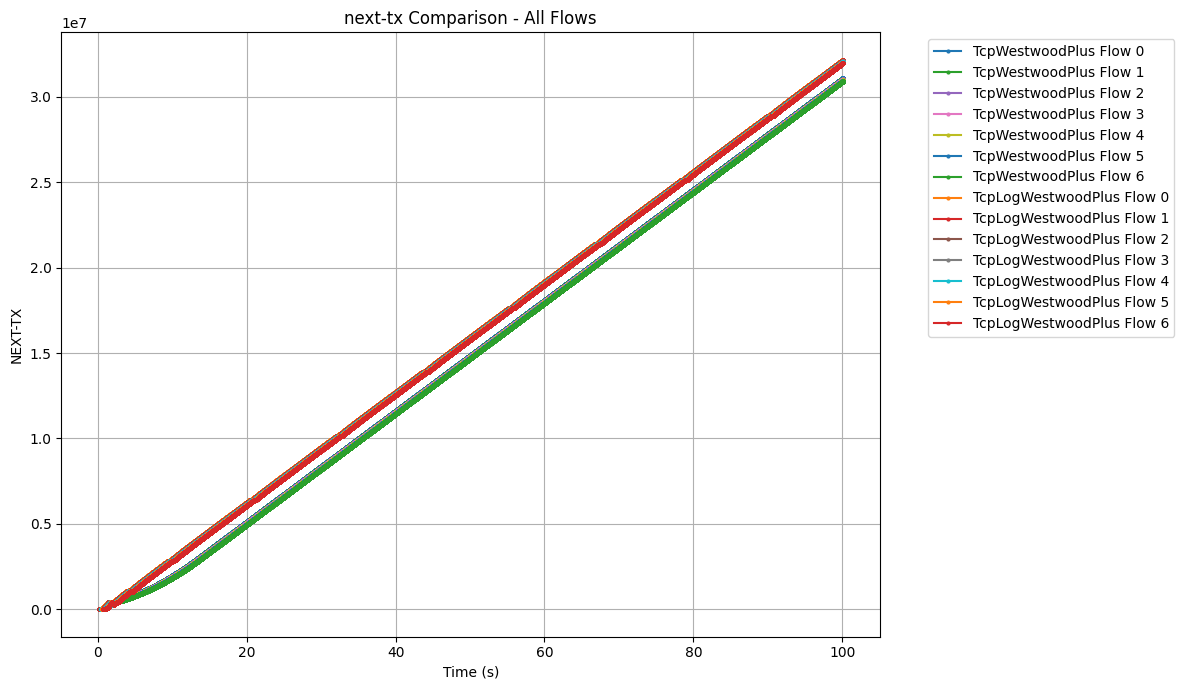
\includegraphics[width=0.95\textwidth]{plots/combined/Veno-WestwoodPlus/flowcombined/next-tx_all_flows_comparison.png}
\caption{Next TX Analysis for TCP Veno vs TCP Westwood+}
\label{fig:Veno-WestwoodPlus_next-tx}
\end{figure}

\newpage

\newpage
\subsection{Retransmission Timeout}
\begin{figure}[H]
\centering
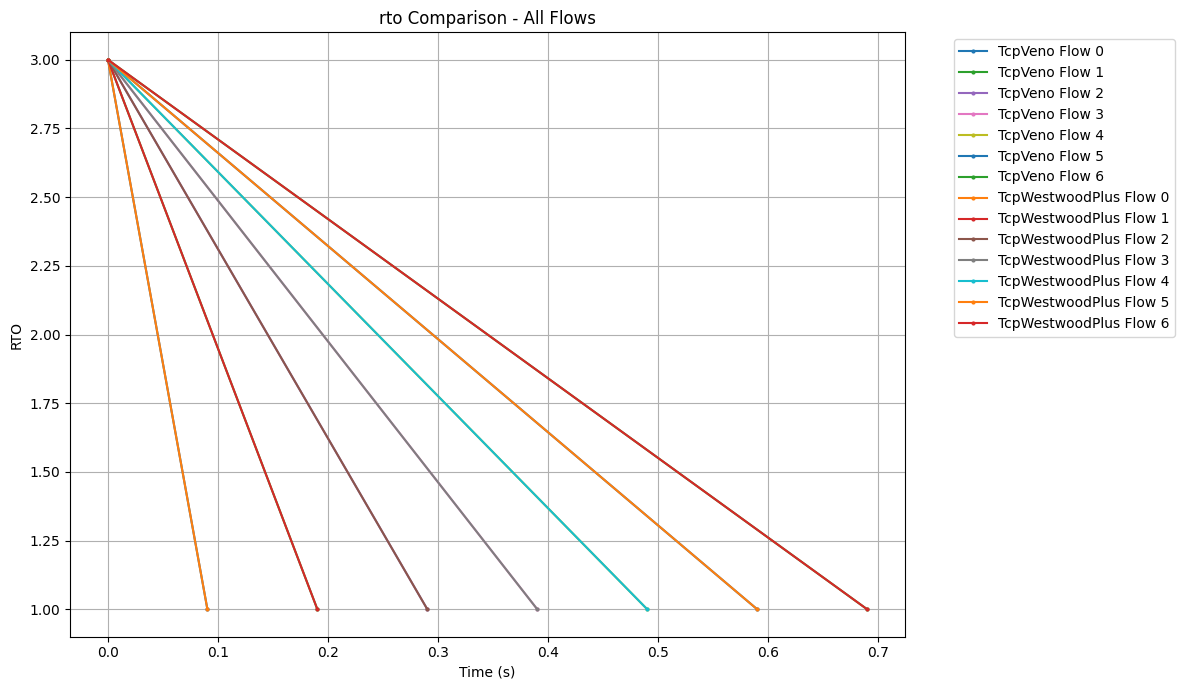
\includegraphics[width=0.95\textwidth]{plots/combined/Veno-WestwoodPlus/flowcombined/rto_all_flows_comparison.png}
\caption{Retransmission Timeout Analysis for TCP Veno vs TCP Westwood+}
\label{fig:Veno-WestwoodPlus_rto}
\end{figure}

\newpage

\newpage
\subsection{Round Trip Time}
\begin{figure}[H]
\centering
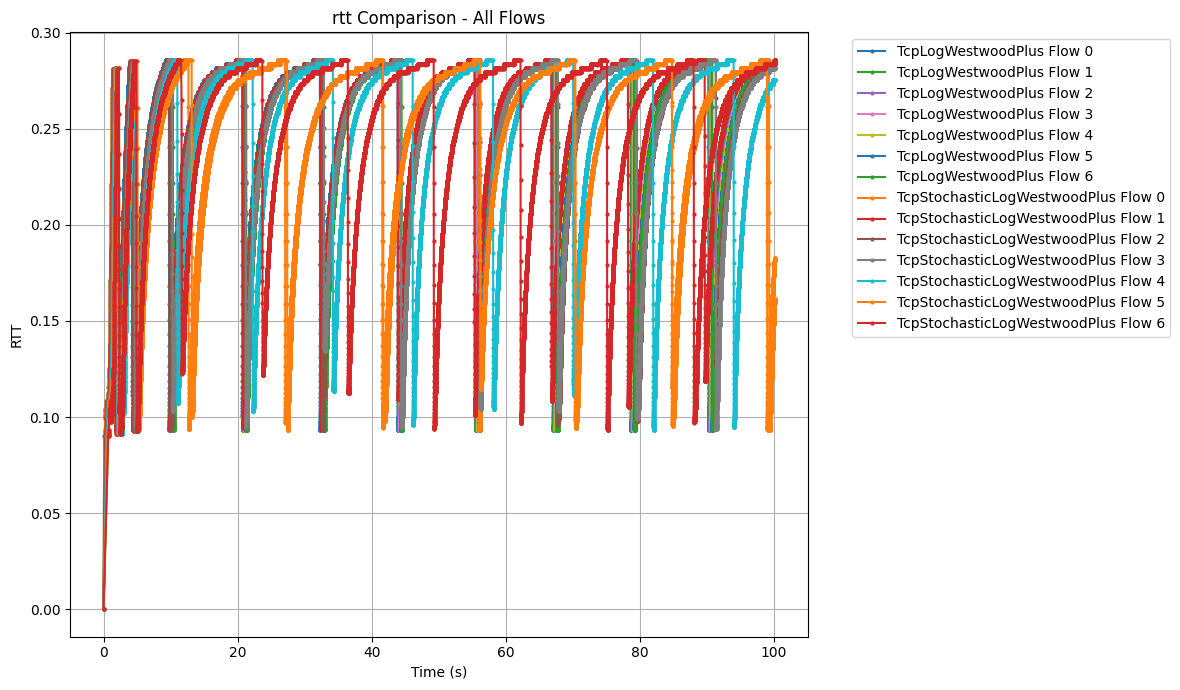
\includegraphics[width=0.95\textwidth]{plots/combined/Veno-WestwoodPlus/flowcombined/rtt_all_flows_comparison.png}
\caption{Round Trip Time Analysis for TCP Veno vs TCP Westwood+}
\label{fig:Veno-WestwoodPlus_rtt}
\end{figure}

\newpage

\newpage
\subsection{Slow Start Threshold}
\begin{figure}[H]
\centering
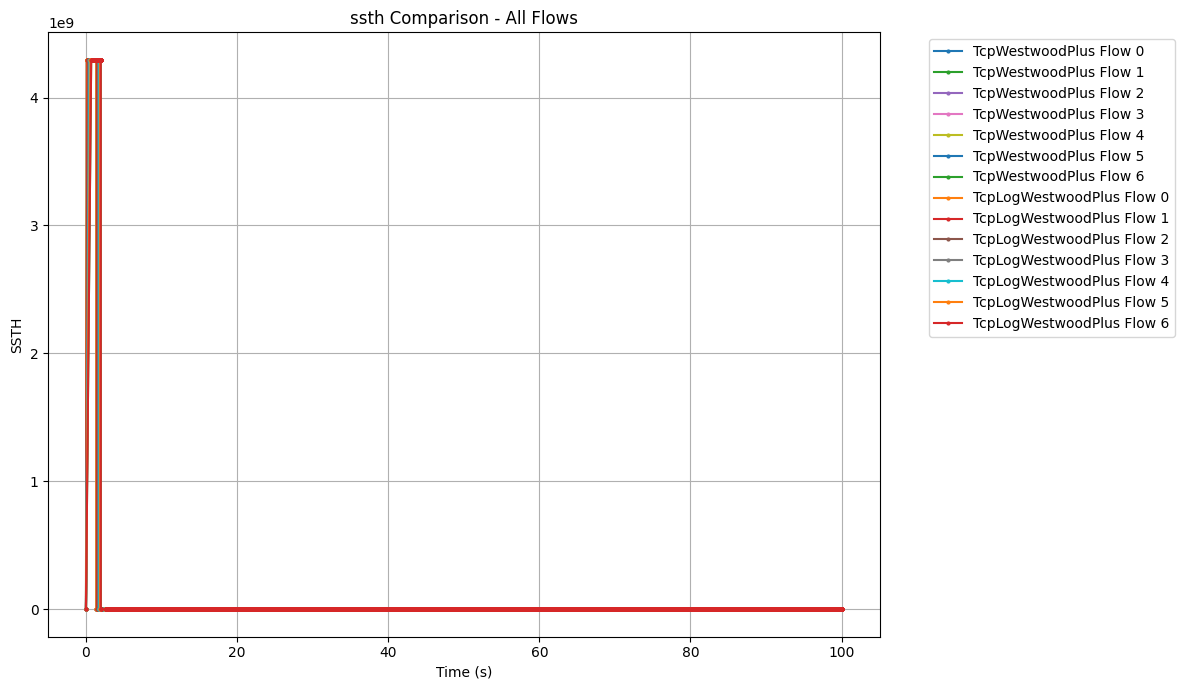
\includegraphics[width=0.95\textwidth]{plots/combined/Veno-WestwoodPlus/flowcombined/ssth_all_flows_comparison.png}
\caption{Slow Start Threshold Analysis for TCP Veno vs TCP Westwood+}
\label{fig:Veno-WestwoodPlus_ssth}
\end{figure}

\newpage

\subsection{Slow Start Threshold (Logarithmic Scale)}
\begin{figure}[H]
\centering
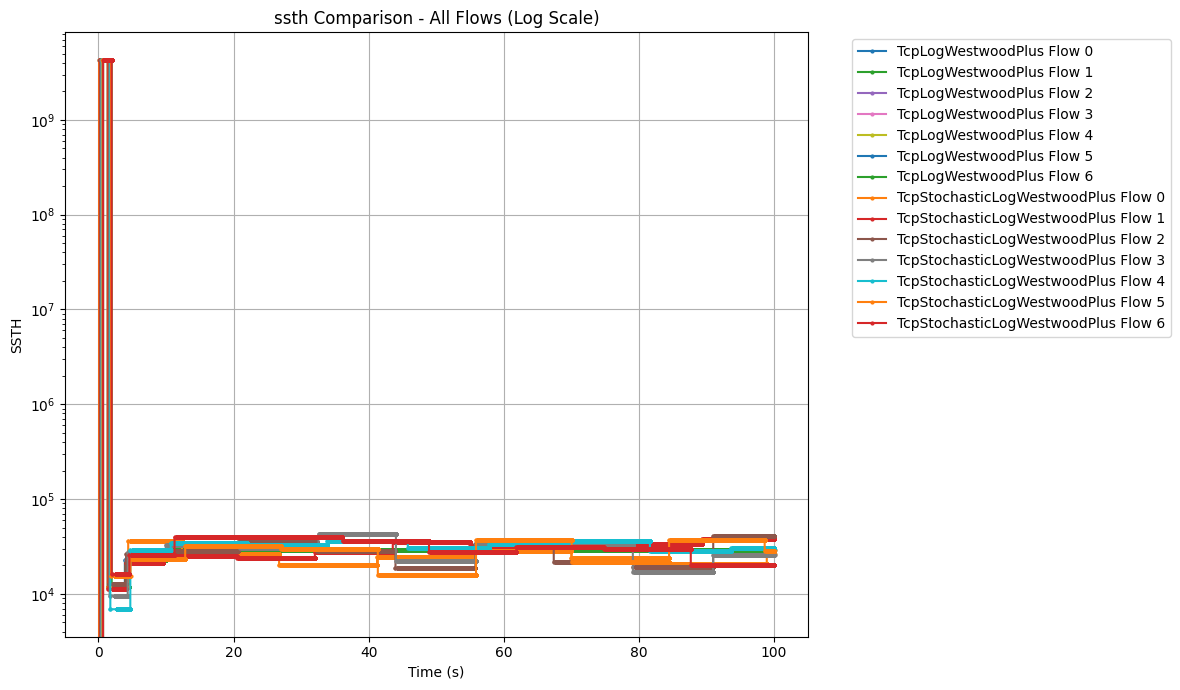
\includegraphics[width=0.95\textwidth]{plots/combined/Veno-WestwoodPlus/flowcombined/ssth_all_flows_comparison_log.png}
\caption{Slow Start Threshold Analysis (Log Scale) for TCP Veno vs TCP Westwood+}
\label{fig:Veno-WestwoodPlus_ssth_log}
\end{figure}

\newpage

\section{TCP Westwood+ vs TCP Log Westwood+}
\noindent Analysis of the impact of logarithmic modifications to TCP Westwood+.


\newpage
\subsection{Congestion Window}
\begin{figure}[H]
\centering
\includegraphics[width=0.95\textwidth]{plots/combined/WestwoodPlus-LogWestwoodPlus/flowaveraged/cwnd_flow_averaged.png}
\caption{Congestion Window Analysis for TCP Westwood+ vs TCP Log Westwood+}
\label{fig:WestwoodPlus-LogWestwoodPlus_cwnd}
\end{figure}

\newpage

\newpage
\subsection{In-Flight Packets}
\begin{figure}[H]
\centering
\includegraphics[width=0.95\textwidth]{plots/combined/WestwoodPlus-LogWestwoodPlus/flowaveraged/inflight_flow_averaged.png}
\caption{In-Flight Packets Analysis for TCP Westwood+ vs TCP Log Westwood+}
\label{fig:WestwoodPlus-LogWestwoodPlus_inflight}
\end{figure}

\newpage

\newpage
\subsection{Next RX}
\begin{figure}[H]
\centering
\includegraphics[width=0.95\textwidth]{plots/combined/WestwoodPlus-LogWestwoodPlus/flowaveraged/next-rx_flow_averaged.png}
\caption{Next RX Analysis for TCP Westwood+ vs TCP Log Westwood+}
\label{fig:WestwoodPlus-LogWestwoodPlus_next-rx}
\end{figure}

\newpage

\newpage
\subsection{Next TX}
\begin{figure}[H]
\centering
\includegraphics[width=0.95\textwidth]{plots/combined/WestwoodPlus-LogWestwoodPlus/flowaveraged/next-tx_flow_averaged.png}
\caption{Next TX Analysis for TCP Westwood+ vs TCP Log Westwood+}
\label{fig:WestwoodPlus-LogWestwoodPlus_next-tx}
\end{figure}

\newpage

\newpage
\subsection{Retransmission Timeout}
\begin{figure}[H]
\centering
\includegraphics[width=0.95\textwidth]{plots/combined/WestwoodPlus-LogWestwoodPlus/flowaveraged/rto_flow_averaged.png}
\caption{Retransmission Timeout Analysis for TCP Westwood+ vs TCP Log Westwood+}
\label{fig:WestwoodPlus-LogWestwoodPlus_rto}
\end{figure}

\newpage

\newpage
\subsection{Round Trip Time}
\begin{figure}[H]
\centering
\includegraphics[width=0.95\textwidth]{plots/combined/WestwoodPlus-LogWestwoodPlus/flowaveraged/rtt_flow_averaged.png}
\caption{Round Trip Time Analysis for TCP Westwood+ vs TCP Log Westwood+}
\label{fig:WestwoodPlus-LogWestwoodPlus_rtt}
\end{figure}

\newpage

\newpage
\subsection{Slow Start Threshold}
\begin{figure}[H]
\centering
\includegraphics[width=0.95\textwidth]{plots/combined/WestwoodPlus-LogWestwoodPlus/flowaveraged/ssth_flow_averaged.png}
\caption{Slow Start Threshold Analysis for TCP Westwood+ vs TCP Log Westwood+}
\label{fig:WestwoodPlus-LogWestwoodPlus_ssth}
\end{figure}

\newpage

\subsection{Slow Start Threshold (Logarithmic Scale)}
\begin{figure}[H]
\centering
\includegraphics[width=0.95\textwidth]{plots/combined/WestwoodPlus-LogWestwoodPlus/flowaveraged/ssth_flow_averaged_log.png}
\caption{Slow Start Threshold Analysis (Log Scale) for TCP Westwood+ vs TCP Log Westwood+}
\label{fig:WestwoodPlus-LogWestwoodPlus_ssth_log}
\end{figure}

\newpage

\section{TCP Log Westwood+ vs TCP Stochastic Log Westwood+}
\noindent Evaluation of stochastic enhancements to Log TCP Westwood+.


\newpage
\subsection{Congestion Window}
\begin{figure}[H]
\centering
\includegraphics[width=0.95\textwidth]{plots/combined/LogWestwoodPlus-StochasticLogWestwoodPlus/flowaveraged/cwnd_flow_averaged.png}
\caption{Congestion Window Analysis for TCP Log Westwood+ vs TCP Stochastic Log Westwood+}
\label{fig:LogWestwoodPlus-StochasticLogWestwoodPlus_cwnd}
\end{figure}

\newpage

\newpage
\subsection{In-Flight Packets}
\begin{figure}[H]
\centering
\includegraphics[width=0.95\textwidth]{plots/combined/LogWestwoodPlus-StochasticLogWestwoodPlus/flowaveraged/inflight_flow_averaged.png}
\caption{In-Flight Packets Analysis for TCP Log Westwood+ vs TCP Stochastic Log Westwood+}
\label{fig:LogWestwoodPlus-StochasticLogWestwoodPlus_inflight}
\end{figure}

\newpage

\newpage
\subsection{Next RX}
\begin{figure}[H]
\centering
\includegraphics[width=0.95\textwidth]{plots/combined/LogWestwoodPlus-StochasticLogWestwoodPlus/flowaveraged/next-rx_flow_averaged.png}
\caption{Next RX Analysis for TCP Log Westwood+ vs TCP Stochastic Log Westwood+}
\label{fig:LogWestwoodPlus-StochasticLogWestwoodPlus_next-rx}
\end{figure}

\newpage

\newpage
\subsection{Next TX}
\begin{figure}[H]
\centering
\includegraphics[width=0.95\textwidth]{plots/combined/LogWestwoodPlus-StochasticLogWestwoodPlus/flowaveraged/next-tx_flow_averaged.png}
\caption{Next TX Analysis for TCP Log Westwood+ vs TCP Stochastic Log Westwood+}
\label{fig:LogWestwoodPlus-StochasticLogWestwoodPlus_next-tx}
\end{figure}

\newpage

\newpage
\subsection{Retransmission Timeout}
\begin{figure}[H]
\centering
\includegraphics[width=0.95\textwidth]{plots/combined/LogWestwoodPlus-StochasticLogWestwoodPlus/flowaveraged/rto_flow_averaged.png}
\caption{Retransmission Timeout Analysis for TCP Log Westwood+ vs TCP Stochastic Log Westwood+}
\label{fig:LogWestwoodPlus-StochasticLogWestwoodPlus_rto}
\end{figure}

\newpage

\newpage
\subsection{Round Trip Time}
\begin{figure}[H]
\centering
\includegraphics[width=0.95\textwidth]{plots/combined/LogWestwoodPlus-StochasticLogWestwoodPlus/flowaveraged/rtt_flow_averaged.png}
\caption{Round Trip Time Analysis for TCP Log Westwood+ vs TCP Stochastic Log Westwood+}
\label{fig:LogWestwoodPlus-StochasticLogWestwoodPlus_rtt}
\end{figure}

\newpage

\newpage
\subsection{Slow Start Threshold}
\begin{figure}[H]
\centering
\includegraphics[width=0.95\textwidth]{plots/combined/LogWestwoodPlus-StochasticLogWestwoodPlus/flowaveraged/ssth_flow_averaged.png}
\caption{Slow Start Threshold Analysis for TCP Log Westwood+ vs TCP Stochastic Log Westwood+}
\label{fig:LogWestwoodPlus-StochasticLogWestwoodPlus_ssth}
\end{figure}

\newpage

\subsection{Slow Start Threshold (Logarithmic Scale)}
\begin{figure}[H]
\centering
\includegraphics[width=0.95\textwidth]{plots/combined/LogWestwoodPlus-StochasticLogWestwoodPlus/flowaveraged/ssth_flow_averaged_log.png}
\caption{Slow Start Threshold Analysis (Log Scale) for TCP Log Westwood+ vs TCP Stochastic Log Westwood+}
\label{fig:LogWestwoodPlus-StochasticLogWestwoodPlus_ssth_log}
\end{figure}

\newpage

\chapter{Conclusions}
\section{Key Findings}
\begin{itemize}
\item Comparative performance of TCP variants
\item Impact of logarithmic modifications
\item Effects of stochastic enhancements
\end{itemize}

\end{document}